\documentclass[onecolumn]{article}
%\usepackage{url}
%\usepackage{algorithmic}
\usepackage[a4paper]{geometry}
\usepackage{datetime}
\usepackage[margin=2em, font=small,labelfont=it]{caption}
\usepackage{graphicx}
\usepackage{mathpazo} % use palatino
\usepackage[scaled]{helvet} % helvetica
\usepackage{microtype}
\usepackage{amsmath}
\usepackage{subfigure}
\usepackage{hyperref}
\hypersetup{colorlinks=true, linkcolor=blue, filecolor=magenta, urlcolor=blue}
\newcommand{\spacecaps}[1]{\textls[200]{\MakeUppercase{#1}}}
\newcommand{\spacesc}[1]{\textls[50]{\textsc{\MakeLowercase{#1}}}}

\title{\spacecaps{Project module report: Argumentation Mining }\\
       \normalsize\spacesc{University of Potsdam, Winter semester 2017/18}}

\author{Oğuz Şerbetci, Maria Stazherova}
\date{\today}

\begin{document}
\maketitle

\begin{abstract}

Structure prediction on ``microtext'' corpus. We used Keras Functional API throughout the project. The code can be found on GitHub at \url{https://github.com/oguzserbetci/argmin2017}.

\end{abstract}


\section{Task \& Data}
Argument mining is the field of study that deals with parsing the structure of the arguments in discourse, such that it eases the successive analysis.

In this project our goal was to predict argumentative structures in the
Argumentative microtext corpus~\cite{peldszus2015annotated}, which contains 112 short argumentative texts
(originally in German and professionally translated to English). Later we received preliminary annotations of the new microtexts
and could incorporate them into the project.

\begin{figure}[h]
    \centering
    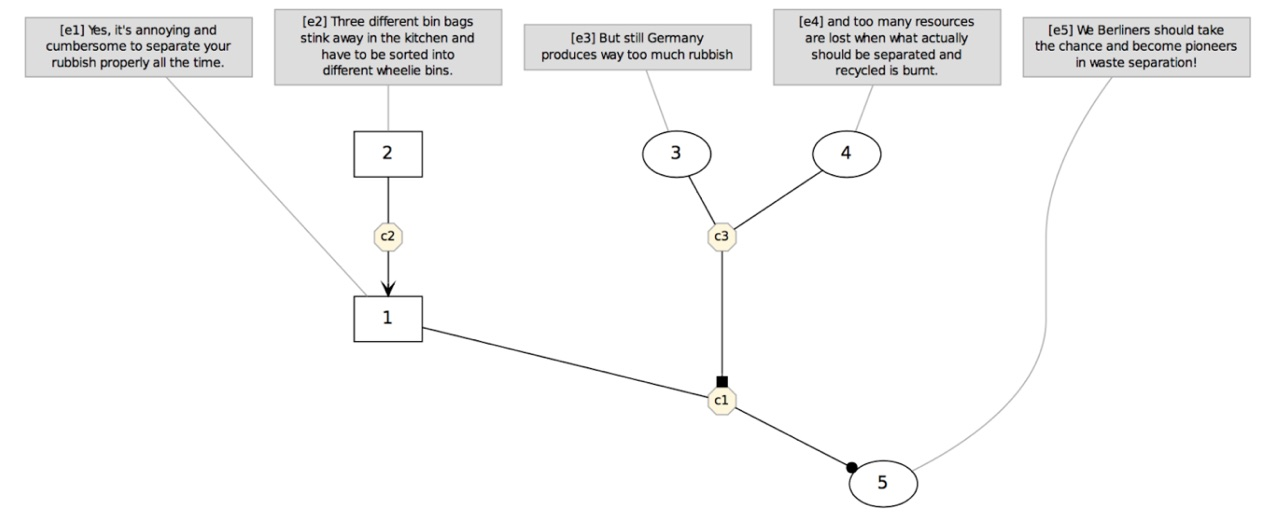
\includegraphics[width=0.8\linewidth]{fig/microtext.jpg}
    \caption{One example from arg-microtext corpus and its argumentation graph.
            \\Round nodes are proponent's nodes, square ones are opponent's nodes.
            The arcs connecting the nodes represent different supporting and attacking moves.}\label{fig:microtext}
\end{figure}

As seen in the figure~\ref{fig:microtext}, each text in the corpus is a single tree made up of argument components (ACs), of which one is the claim and the rest premises.
We decided to concentrate on two tasks: classifying the type of an AC (claim or premise), and determining the links between ACs.

\section{Approach}
\subsection{Inspiration}
Having found the paper ``Here's My Point: Joint Pointer Architecture for Argument Mining'' by Potash et al.~\cite{potash2017here}, we agreed that it
would be good to try and reproduce the architecture and results from this paper, especially because the authors claimed they achieved
state-of-the-art results. The authors use a Pointer Network which is a modification of seq2seq (sequence-to-sequence) architecture with attention.

The pointer network architecture is extended in two ways.
First, to account for the large and sparse AC representations authors add fully-connected layers before the encoder and decoder LSTM inputs.
Second, to improve performance they add an auxiliary task for predicting if an AC is the claim or a premise.
Multi-task learning in deep neural networks has been shown to perform better in comparison to single task~\cite{multi}, which this work further demonstrates.

\subsection{Architecture}
The architecture is a seq2seq model as depicted in~\autoref{fig:seq2seq}.
For brevity let us leave out the fully connected layers before the inputs of the encoder and the decoder.
At each time step, an AC is input into the encoder which results in hidden state $e_i$.
Each $e_i$ is used to predict the type $T_i$ of the $\text{AC}_i$.

\begin{align*}
    z_i = W_{\text{cls}} e_i + b_{\text{cls}}\\
    p(T_i|E_i;\Theta) = \text{softmax}(z_i).
\end{align*}


After the final AC has been input into the encoder, the decoder has its first time step.
The first input to the decoder is always the special start token and results with the hidden state $d_1$.
At each decoder time step the modified attention mechanism predicts a link $D_i$ as follows:
\begin{align*}
    u_j^i &= v^\top \tanh(W_1e_j + W_2d_i)\\
    p(D_i|D_1,\dots,D_{j-1},E) &= \text{softmax}(u^i).
\end{align*}

Predictions are depicted in~\autoref{fig:type} and~\ref{fig:link}.

\begin{figure}[h]
    \centering
    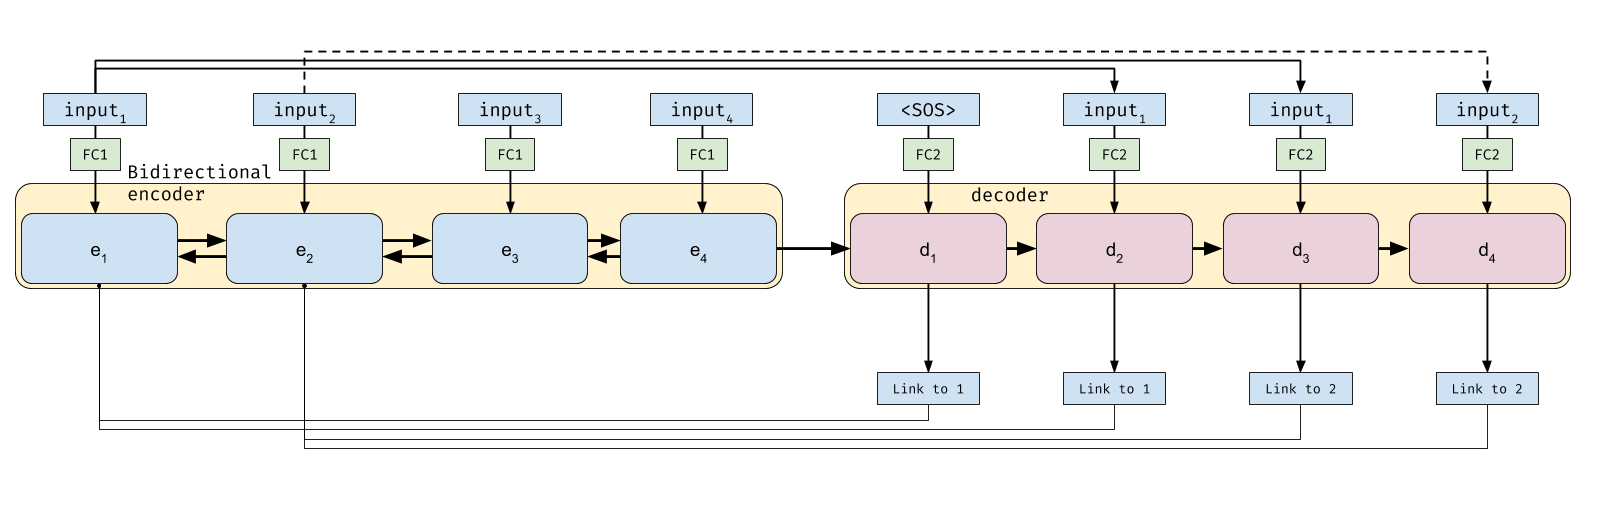
\includegraphics[width=0.95\linewidth]{fig/seq2seq.png}
    \caption{Architecture of seq2seq model from the paper.}\label{fig:seq2seq}
\end{figure}

\begin{figure}[h]
    \centering
    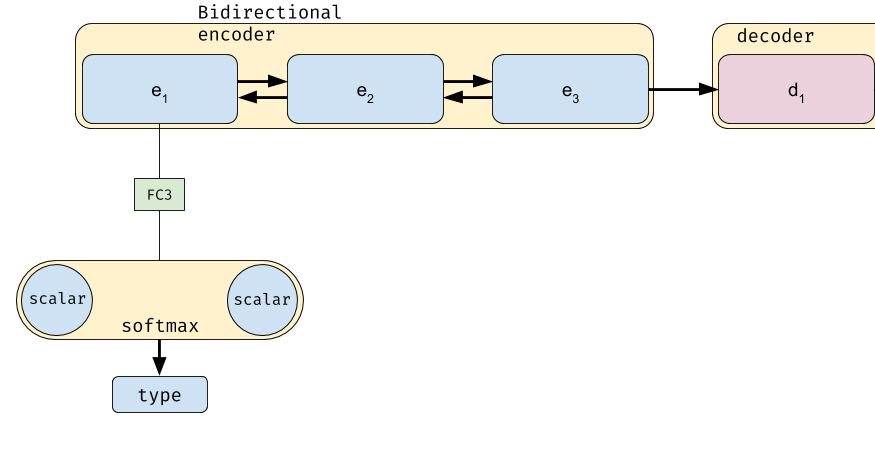
\includegraphics[width=0.8\linewidth]{fig/type.png}
    \caption{Diagram of the model for predicting type of an $\text{AC}_1$.}\label{fig:type}
\end{figure}

\begin{figure}[h]
    \centering
    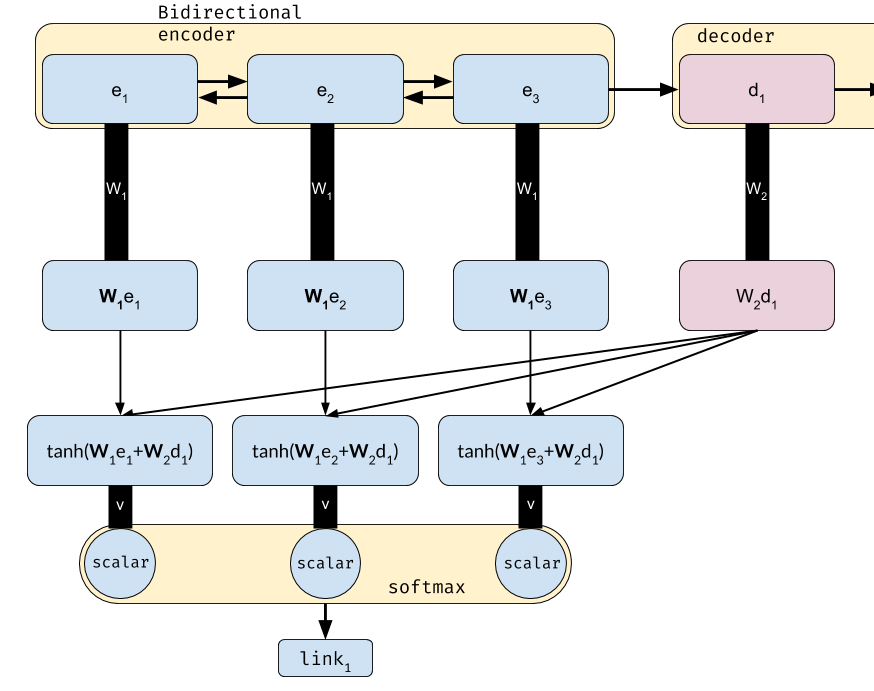
\includegraphics[width=0.8\linewidth]{fig/link.png}
    \caption{Diagram of the model for predicting the outgoing link from the $\text{AC}_1$.}\label{fig:link}
\end{figure}

\subsection{Organisation}
We have set milestones to enforce deadlines.
In milestone 1, we have implemented the data preprocessing and creating simple bag-of-words vector representations of argument components.
After that we implemented a pointer network with one-directional encoder for the single task (determining the links between ACs) without the fully connected layer at inputs.
We sticked to using dropout, as it was applied in the paper~\cite{potash2017here}.
However, because the paper didn't specify where the dropout should be used, we have to 

In milestone 2, we extended the architecture with the fully-connected inputs and the bidirectional LSTM for the encoder.
Moreover, we have added all applicable features to AC representation from the paper: structural feature
(binary, is the AC the first one in text or not), bag-of-words over the whole data and embedding representations (average, min and max pooling
of word vectors\footnote{We have used \href{https://github.com/explosion/spacy-models/releases/tag/en_vectors_web_lg-2.0.0}{spacy} word vectors.} of tokens).

In milestone 3, we moved further on implementing the joint model architecture with an additional task of classifying the type of AC (claim or premise).

During development, we have used 5-fold cross-validation for evaluation and inspection of our implementation.
Some things we had to try out was using regularization, where to apply dropout and the seq2seq architecture.
The regularization did not improve performance when applied as an addition to dropout.
Strictly using l2 regularization also performed worse compared to dropout.
We found that dropout should be strictly applied to LSTMs and nowhere else.

\subsection{Challenges}
While working on the project, we encountered some difficulties and made some errors that we then corrected. The first one
was to think of the proper way to pad input sequences so that they have the same length.

Another mistake we did was to calculate the evaluation metrics wrong.
We have calculated the f1 score not as a binary classification of absence and presence of links, instead a categorical one.
This has resulted in significantly worse results which led us to tinker with our architecture and even implement it in pytorch from scratch.

This mistake and its correction has been a great learning for us, however, we note that the binary measure makes the results look much better than they are,
since by definition for $n$ ACs the network gets $n-2$ absence of links for correct.

\section{Results}
To compare our results we did a single 10-fold cross validation. Our results and the results from~\cite{potash2017here} can be seen in~\autoref{tab:results}.
Only additional configuration we present is to apply class weights into the loss calculation and using the new extended corpus.
We were motivated to use class weights because of the highly skewed link distribution across the corpus as seen in~\autoref{fig:skew}.

\begin{figure}[h]
    \centering
    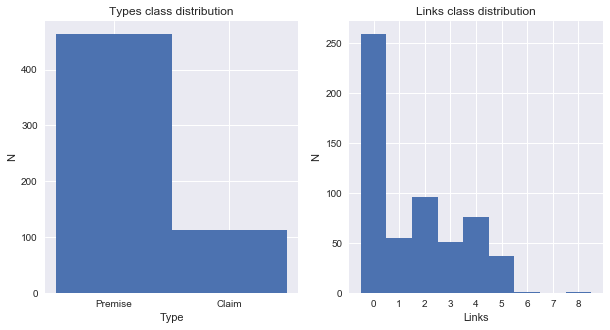
\includegraphics[width=0.4\linewidth]{fig/dist.png}
    \caption{Distribution of links.}\label{fig:skew}
\end{figure}

\section{Conclusion}
future ideas and improvements

\nocite{*}
\bibliographystyle{plain}
\bibliography{references}
\end{document}
